\begin{frame}
\frametitle{Main Application Areas for CP}
\begin{itemize}
\item Scheduling
\item Product Configuration
\item Rostering and Assignment
\item Software/Hardware Design and Testing
\item Transportation
\end{itemize}
\end{frame}

\section{Scheduling}

\begin{frame}
\frametitle{Scheduling Demo}
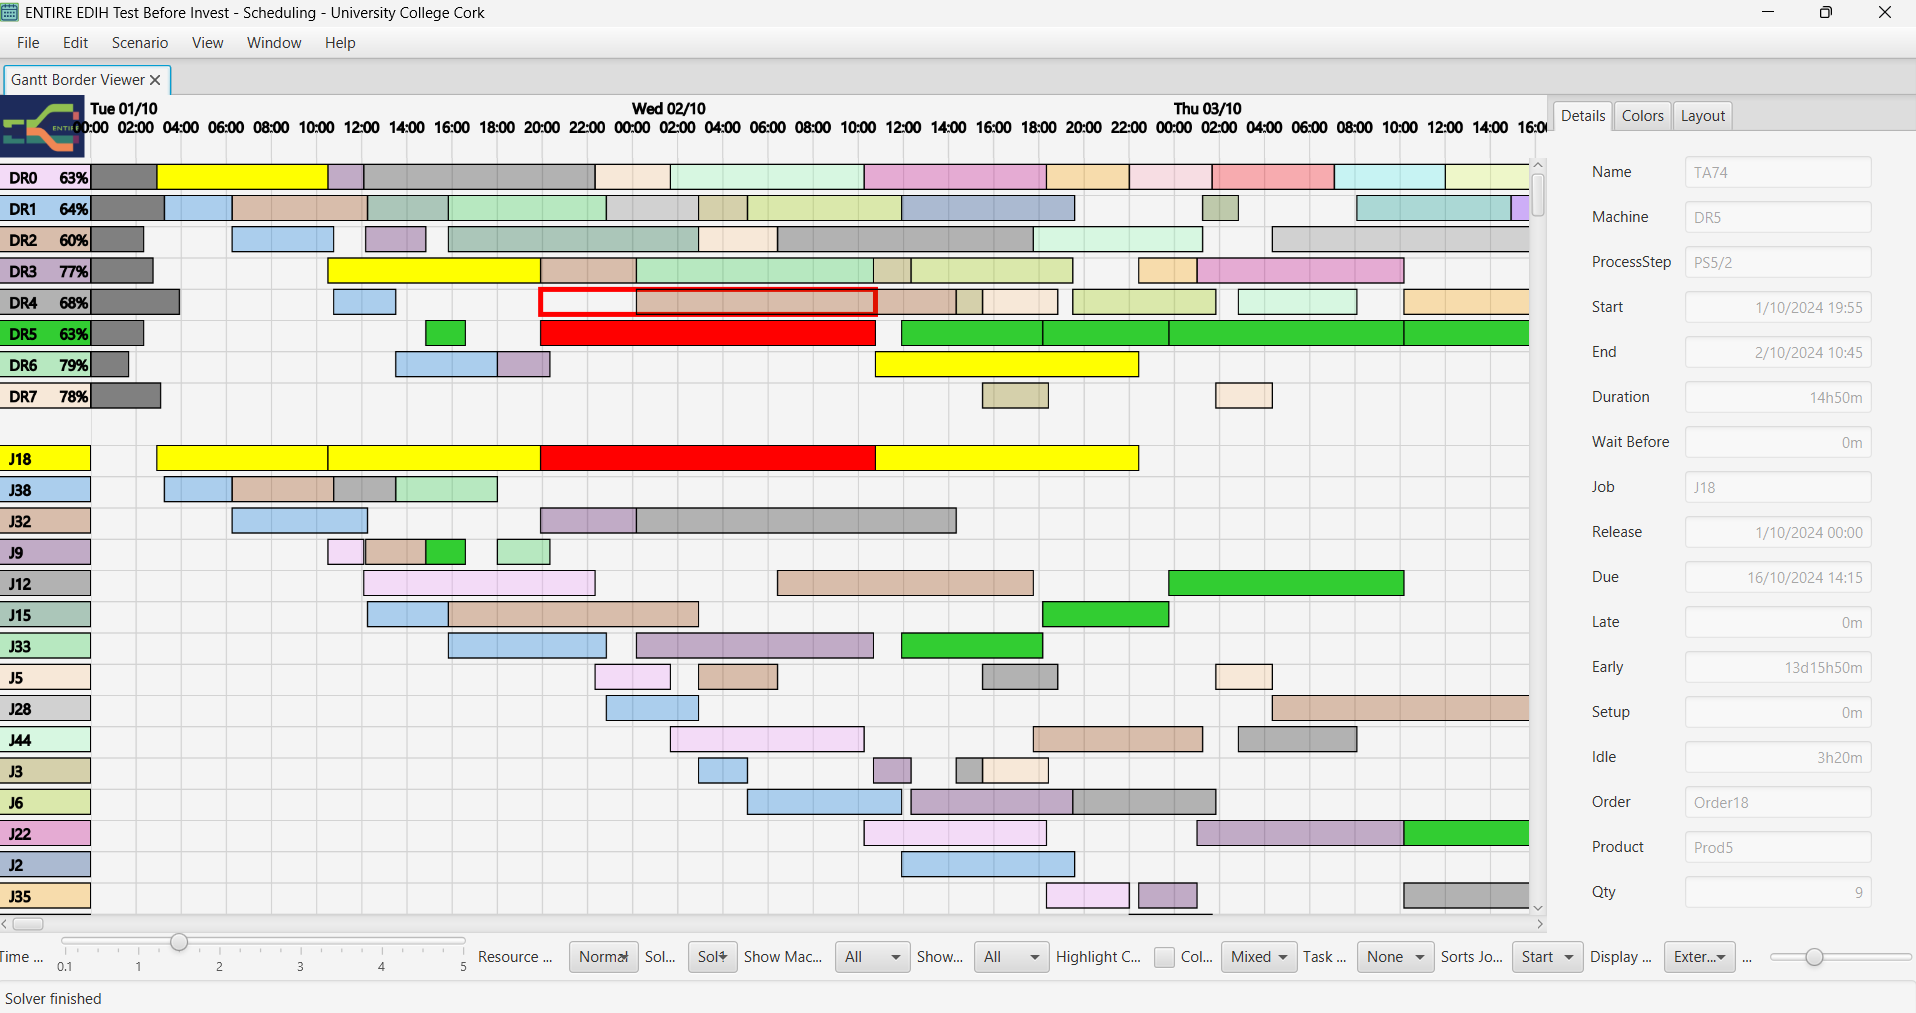
\includegraphics[width=12cm]{images/demoscheduling}
\end{frame}

\begin{frame}
\frametitle{More on Scheduling}
\begin{itemize}
\item Later in this presentation
\item One hour talk in the \href{http://schedulingseminar.com}{Scheduling Seminar} series
\item Video \url{https://www.youtube.com/embed/6fSRT64XE9w?si=B-hcivmO__q9fapD}
\item Slides \url{https://schedulingseminar.com/presentations/schedulingseminar_helmutsimonis.pdf}
\end{itemize}
\end{frame}

\section{Configuration}

\begin{frame}
\frametitle{Product Configuration}
\begin{itemize}
\item Used for semi-custom products
\item Product consist of many different components
\item Many choices for each component type from a catalog
\item Strong constraints between different components
\begin{itemize}
\item Power
\item Bandwidth
\item Space
\item Thermal limits
\end{itemize}
\item Overall objectives: cost, power, space
\end{itemize}
\end{frame}

\begin{frame}
\frametitle{Configuration Example: Railway Signalling (Siemens Austria)}
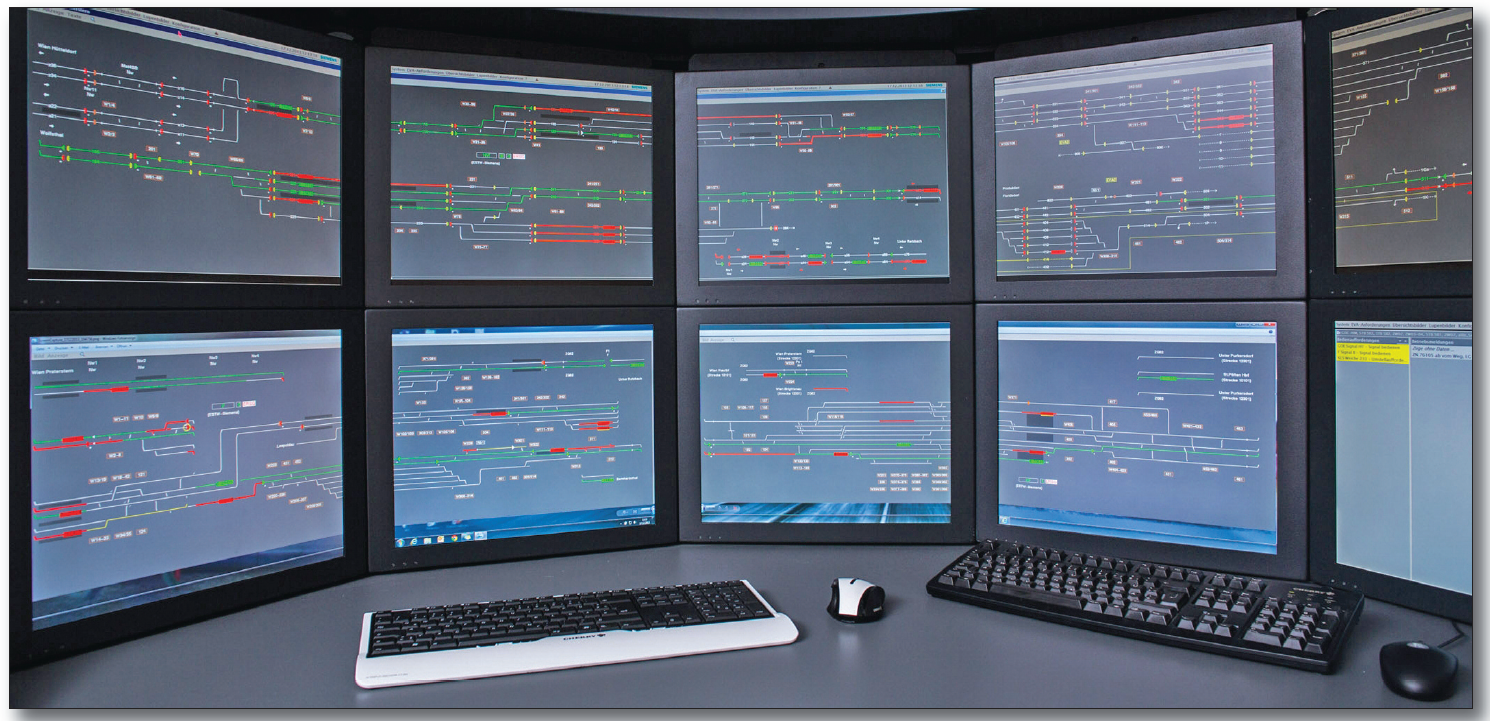
\includegraphics[width=12cm]{images/stellwerkgui}

{\tiny from Falkner  et al, 2016}
\end{frame}

\begin{frame}
\frametitle{Configuration Example: Configurable Hardware (Siemens Austria)}
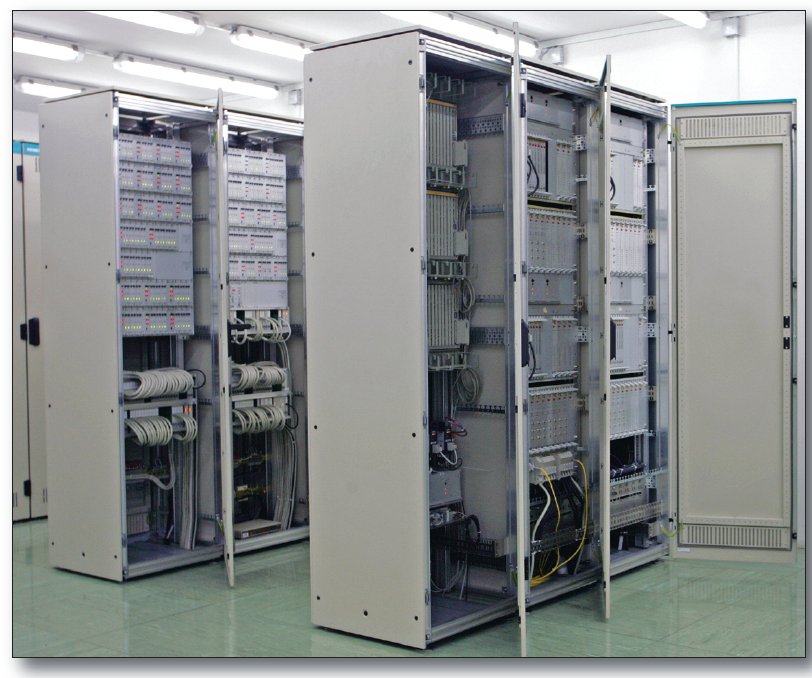
\includegraphics[width=8cm]{images/stellwerkhardware}

{\tiny from Falkner  et al, 2016}
\end{frame}

\begin{frame}
\frametitle{Configuration Modelling}
\begin{itemize}
\item Variables describing alternative component choices
\item Properties of components described by \texttt{table} constraints
\item Linear constraints for global properties
\item \texttt{bin-packing} constraints for rack space
\item \texttt{diffn} constraint for non-overlap in 3D space
\item Multi-objective optimization
\end{itemize}
\end{frame}

\begin{frame}
\frametitle{To learn more}
\begin{itemize}
\item Falkner et al, 2016: Twenty-Five Years of Successful Application of Constraint Technologies at Siemens
\item Erik Cervin-Edin, 2025: Lessons Learnt from Developing \& Maintaining the World's Largest CP Model Using MiniZinc
\item Ulrich Junker, Chapter 24: Configuration, Handbook of Constraint Programming
\end{itemize}
\end{frame}


\section{Rostering}

\begin{frame}
\frametitle{Rostering Demo}
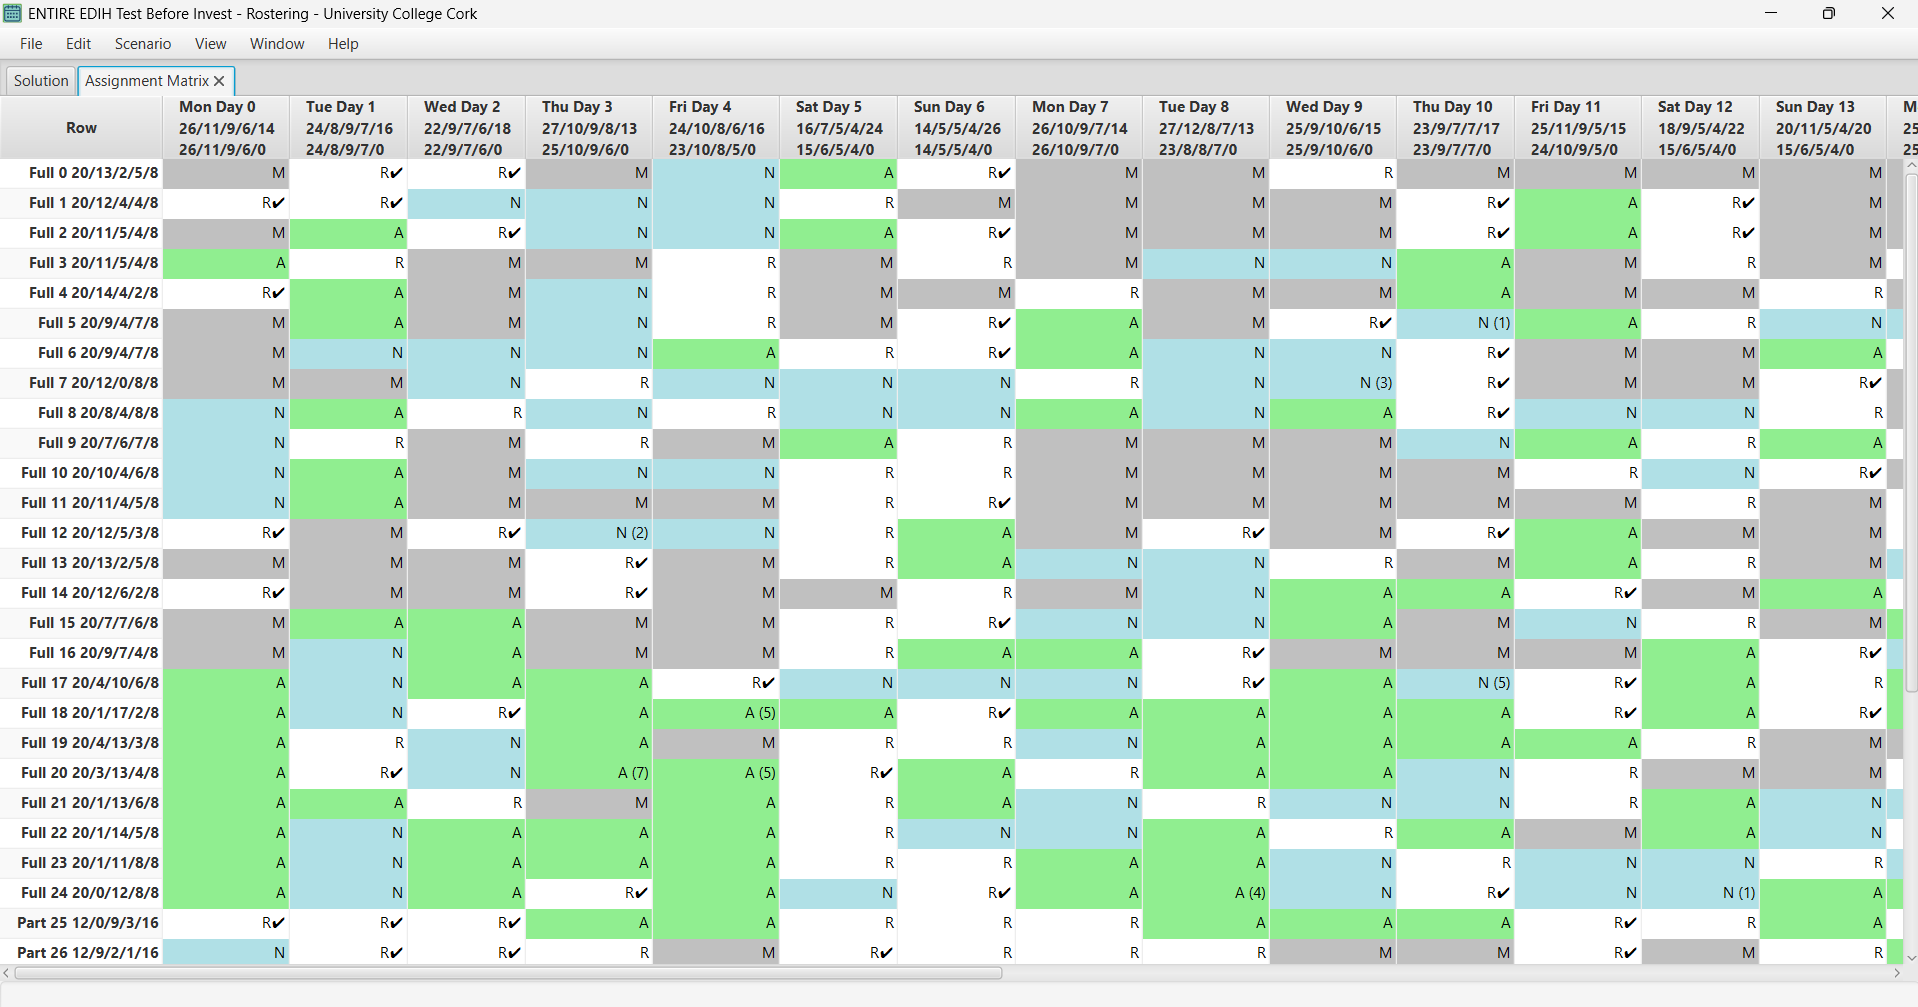
\includegraphics[width=12cm]{images/demorostering}
\end{frame}

\begin{frame}
\frametitle{Rostering}
\begin{itemize}
\item State-of-the-art: Klapperstueck et al, CP 2026: CrewAId: Interactive Optimisation for Human-In-The-Loop Crew Rostering and Rerostering
\item Older: Ernst et al, EJOR 2004: Staff scheduling and rostering: A review of applications, methods and model
\end{itemize}
\end{frame}


\section{Timetabling}

\begin{frame}
\frametitle{Timetabling Demo}
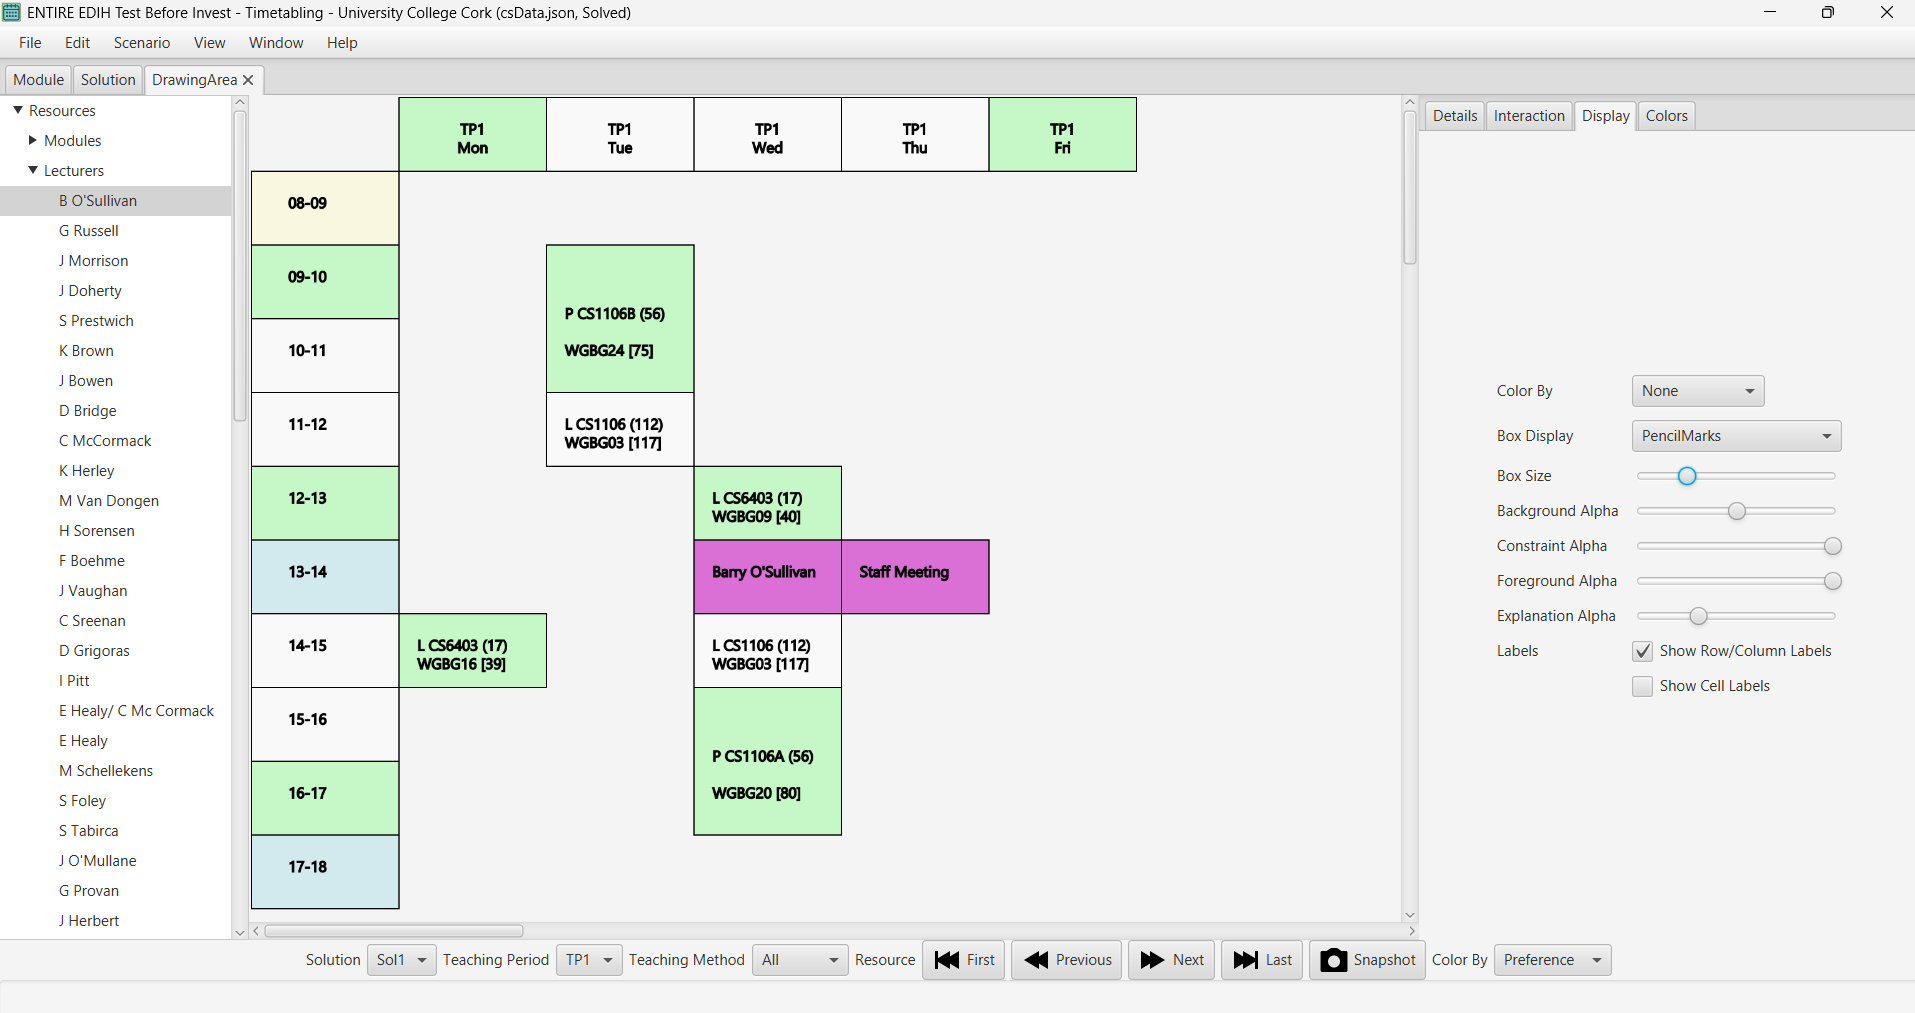
\includegraphics[width=12cm]{images/demotimetabling}
\end{frame}

\begin{frame}
\frametitle{Timetabling}
\begin{itemize}
\item School timetabling
\begin{itemize}
\item Start with Demirovi\`{c}, E., Stuckey, P.J. (2018). \href{https://link.springer.com/chapter/10.1007/978-3-319-93031-2_10}{Constraint Programming for High School Timetabling: A Scheduling-Based Model with Hot Starts}. CPAIOR 2018.
\end{itemize}
\item University timetabling
\begin{itemize}
\item Classic: H.J. Goltz, 1999: University Timetabling using Constraint Logic Programming
\end{itemize}
\item Exam timetabling
\begin{itemize}
\item Good introduction: S. Hamilton, MSc Thesis 2022: Constraint Programming Models For Real-World Examination Scheduling
\end{itemize}
\end{itemize}
\end{frame}

\section{Test/Verification}

\begin{frame}
\frametitle{Test/Verification}
\begin{itemize}
\item Not my area of expertise
\item Specialised CP solvers
\begin{itemize}
\item New domain types, e.g. uint32
\item New constraints, e.g. integer overflow arithmetic
\end{itemize}
\item To learn more: Arnaud Gotlieb video \url{https://www.youtube.com/watch?v=E1Seayx3eXU}
\end{itemize}
\end{frame}

\section{Transportation}

\begin{frame}
\frametitle{Transport Example: TACT}
\begin{itemize}
\item Transporting chickens and turkeys from farms to factory
\begin{itemize}
\item Source of Chicken McNuggets in UK
\end{itemize}
\item Sun Valley Food (Cargill), Hereford, UK
\item Primary objective: Keep factory supplied with birds
\item Multi-resource transport problem
\begin{itemize}
\item Catching teams
\begin{itemize}
\item Drive to farm, catch birds, put in cages, put cages on trucks, go to next farm
\end{itemize}
\item Drivers
\begin{itemize}
\item Drive to farm, load truck with forklift, drive to factory, unload, clean truck, next trip
\end{itemize}
\item Trucks
\begin{itemize}
\item Different vehicle sizes/capacity depends on temperature
\end{itemize}
\end{itemize}

\end{itemize}
\end{frame}

\begin{frame}
\frametitle{Producer/Consumer Constraint for Factory}
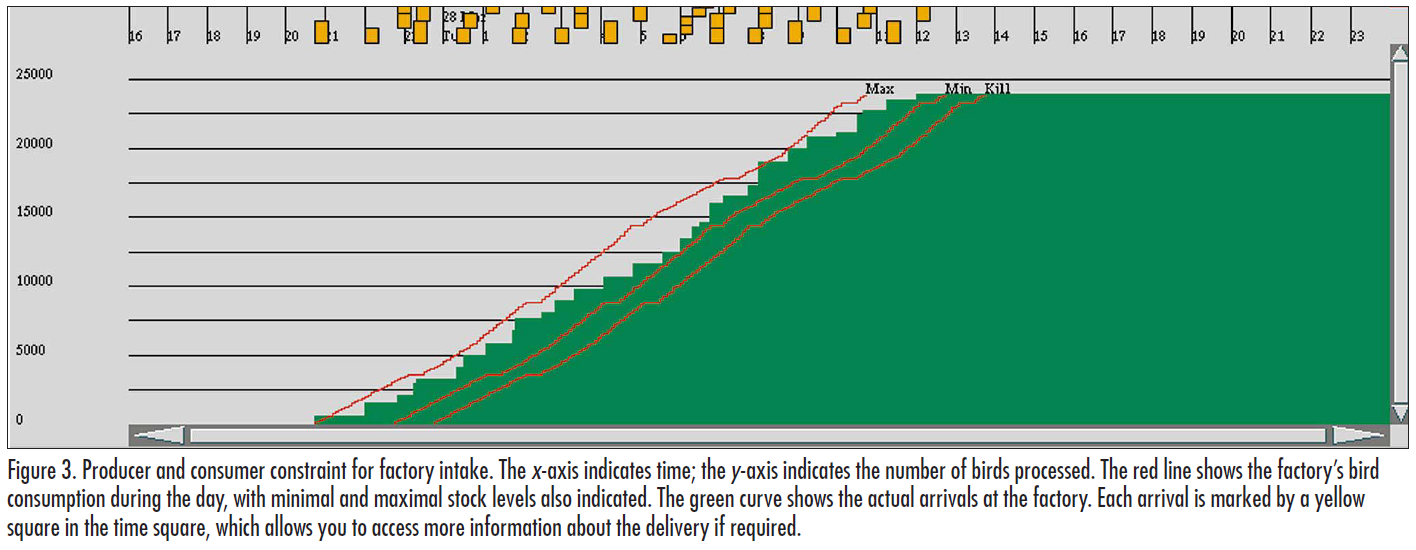
\includegraphics[width=14cm]{../summerschool2026/images/producerconsumer}
\begin{itemize}
\item Do not run factory out of birds!
\item Do not deliver birds too early
\end{itemize}
\end{frame}

\begin{frame}
\frametitle{Order Book}
\begin{columns}
\begin{column}{0.5\textwidth}
\begin{itemize}
\item All trucks/drivers start/end at depot
\item Schedule multiple trips to farms
\begin{itemize}
\item Plan correct number of trips to get all birds from farm
\item Number of trip depends on lorries used
\end{itemize}
\item Transport birds to factory
\item Some transfers between farms
\end{itemize}
\end{column}
\begin{column}{0.5\textwidth}
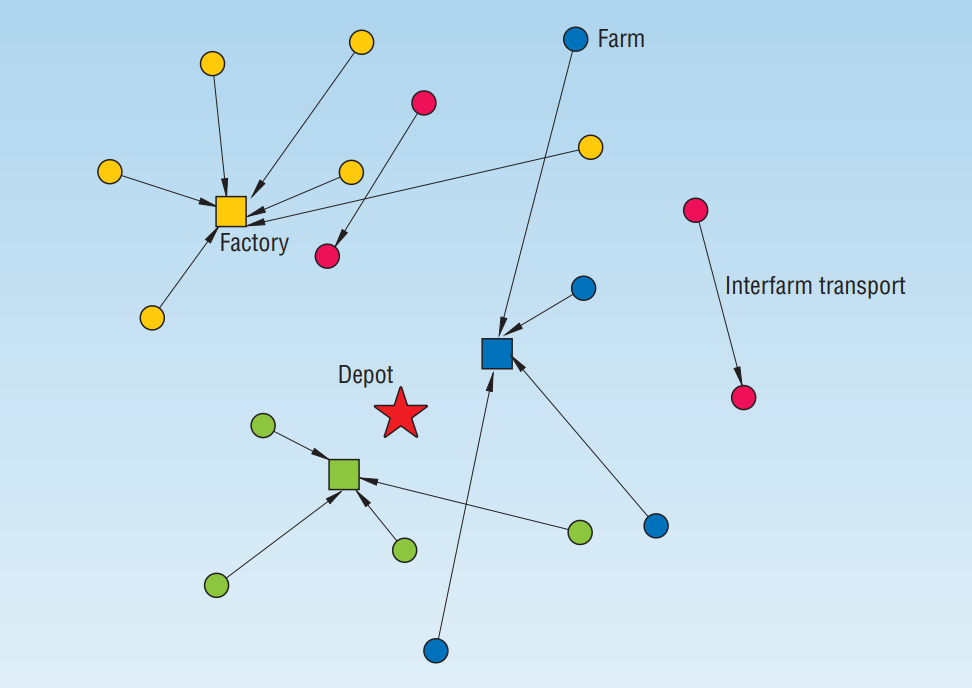
\includegraphics[width=\textwidth]{../summerschool2026/images/orderbook}
\end{column}
\end{columns}
\end{frame}

\begin{frame}
\frametitle{Driver Assignment}
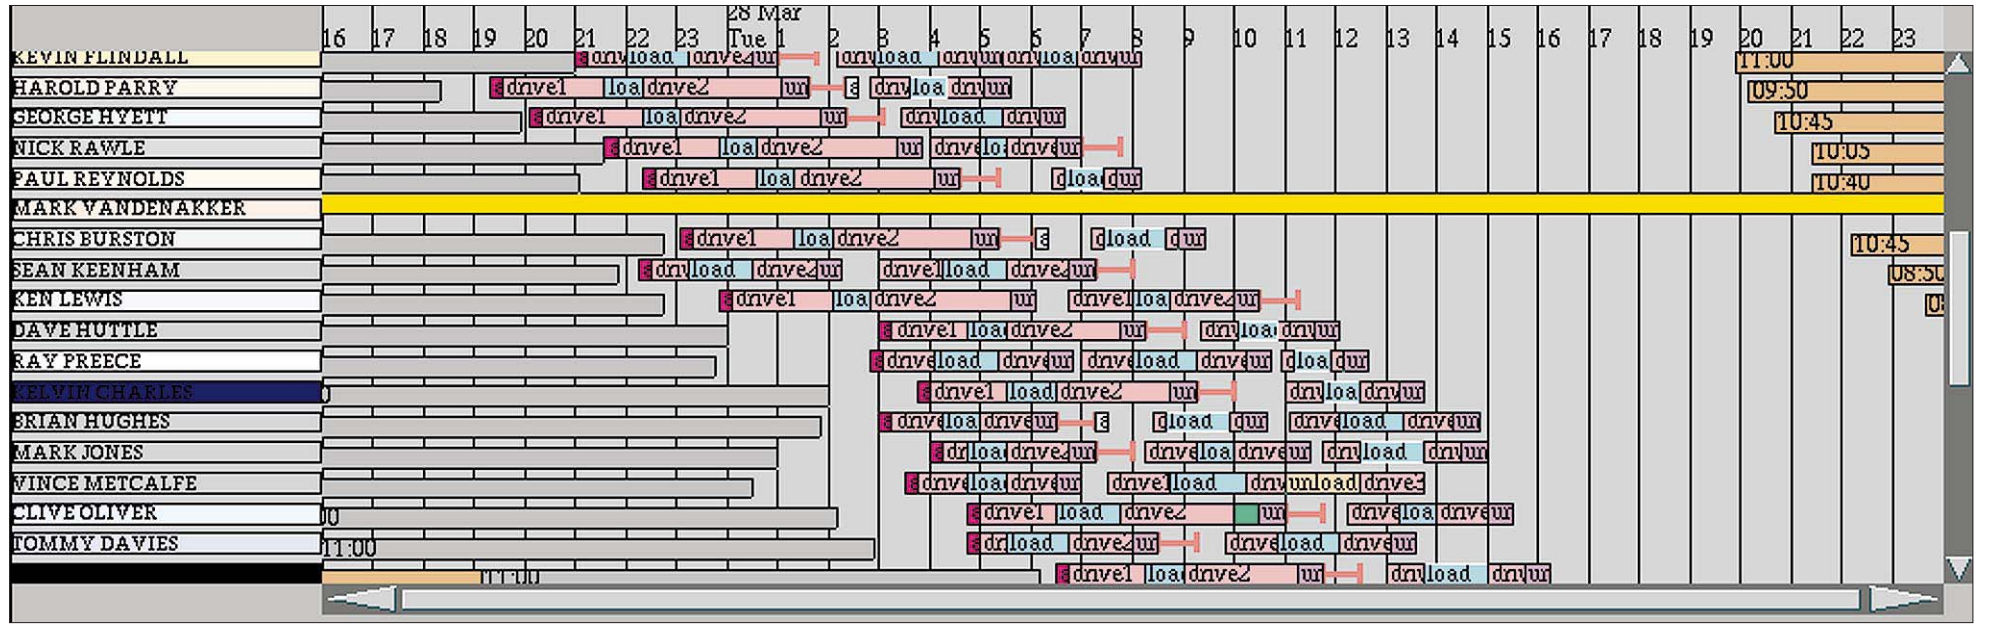
\includegraphics[width=12cm]{../summerschool2026/images/driverassignment}
\begin{itemize}
\item Drivers make 2-4 round trips per day
\item Extra truck/drivers needed for peak demand (cost!)
\item Schedule of one day influences next day (legal rest periods)
\end{itemize}
\end{frame}

\begin{frame}
\frametitle{Truck Assignment}
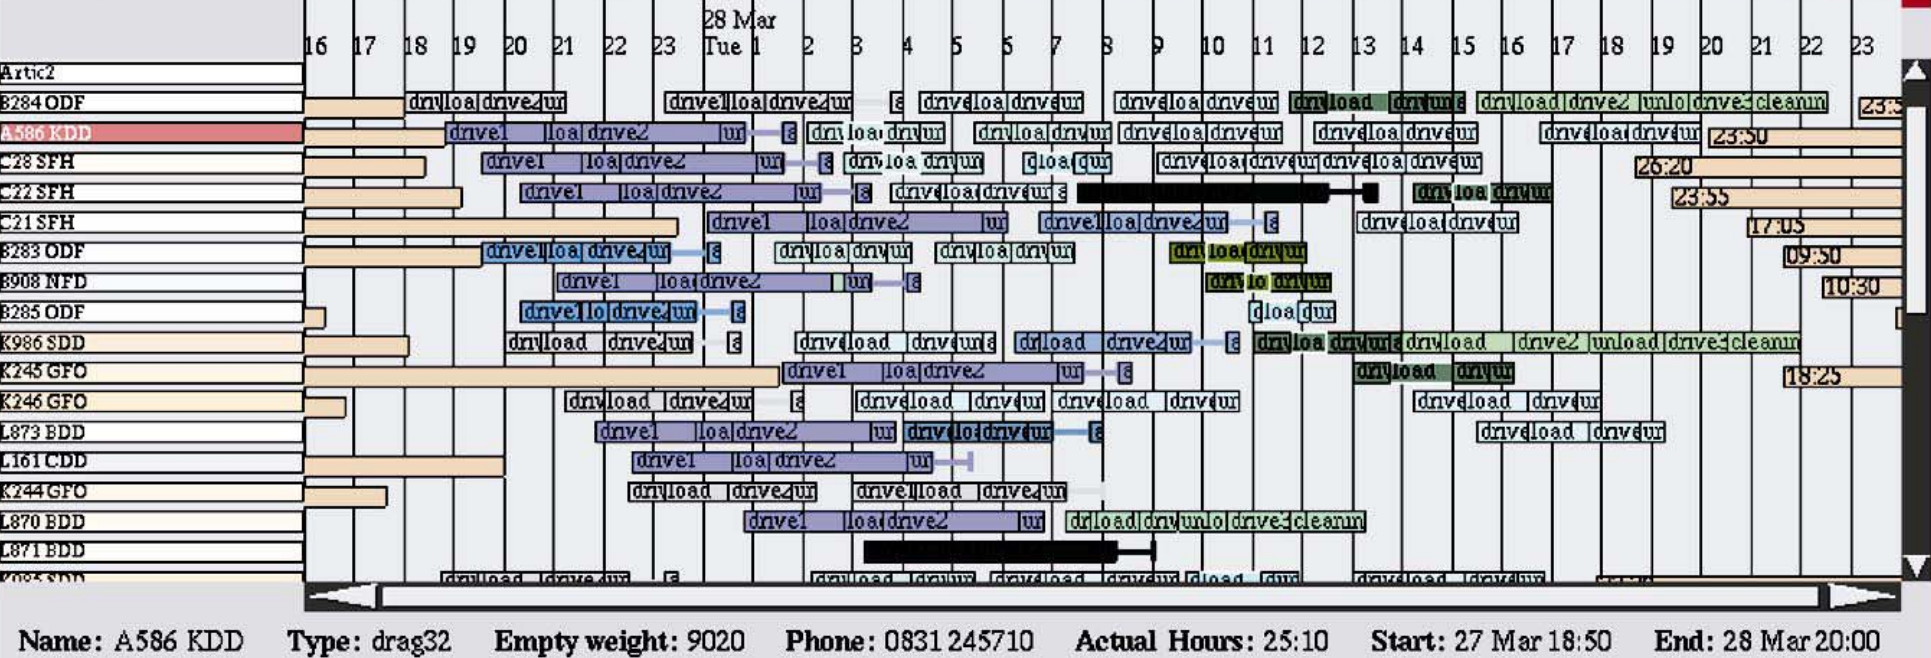
\includegraphics[width=12cm]{../summerschool2026/images/truckassignment}
\begin{itemize}
\item Restrictions of lorry size on certain farms
\item Provide correct transport capacity to get all birds from farms
\item Transport of fork-lifts on truck
\end{itemize}
\end{frame}

\begin{frame}
\frametitle{System}
\begin{itemize}
\item Developed by COSYTEC with CHIP
\item GUI connected to solver and commercial systems
\item Turn-key solution for manager
\item Flexible interactive tool for scheduling expert
\item To learn more: Simonis et al, 2000: Constraint Handling in an Integrated Transportation Problem.
\item More modern solver: Delecluse et al., CP 2022, \href{https://drops.dagstuhl.de/entities/document/10.4230/LIPIcs.CP.2022.19}{Sequence Variables for Routing Problems}

\end{itemize}
\end{frame}

